\section{Data Preprocessing}


\subsection{Data Sources}

This research draws from a range of publicly available datasets with a varied scope of visuals such as animal faces and flowers. The datasets are popular for generating and attribute-editing applications because of their quality and well-labeled categories. For the purpose of this research's emphasis on few-shot image synthesis, only a minority of the images from each dataset are employed. Specifically, a minimal set of representative samples per class are sampled to replicate the few-shot learning situation. The datasets used are:

\begin{enumerate}
    \item \textbf{FUNIT Animal Faces Dataset}
    \begin{figure}[ht]
        \centering
        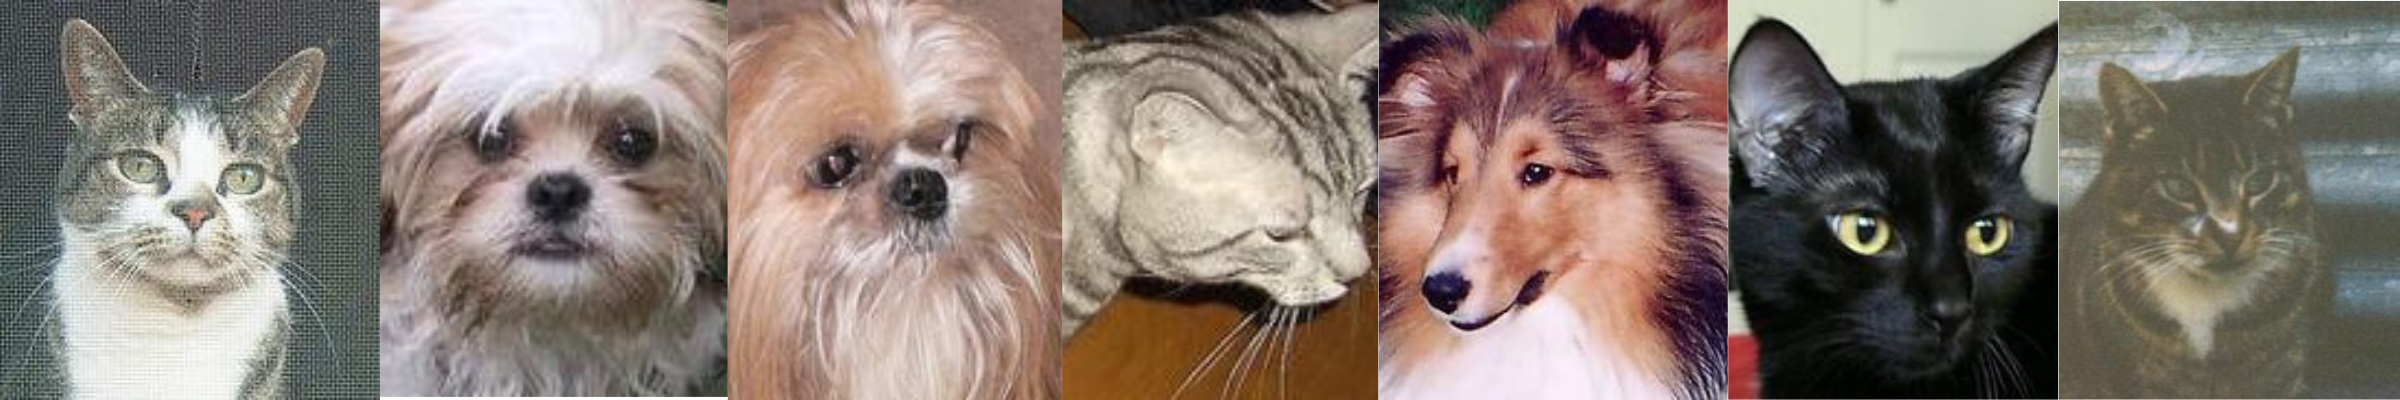
\includegraphics[width=0.9\linewidth]{images/funit_animal_faces_dataset.png}
        \caption{\textit{Sample images from the FUNIT Animal Faces dataset. Source: \citep{liu2019few}}}
        \label{fig:FUNIT_animal_faces}
    \end{figure}

    Figure~\ref{fig:FUNIT_animal_faces} shows representative samples from the FUNIT Animal Faces dataset. The dataset is comprised of 117,484 512~\(\times\)~512 
    resolution high-quality animal face images and is organized in 149 classes (each class is one animal species). Each domain includes a diverse range 
    of species and breeds, ensuring variation in appearance while maintaining consistent facial alignment to support generative model training. The images were 
    curated from openly available sources and standardized in resolution and alignment, with the eyes centrally positioned to provide consistency for learning. 
    A subset of the images is reserved as a test set, with the remainder used for training. The diversity and quality of the FUNIT Animal Faces dataset make it 
    a strong benchmark for generative and attribute-editing models in few-shot settings \citep{liu2019few}.

    \item \textbf{102 Flower (Flowers)}
    \begin{figure}[ht]
        \centering
        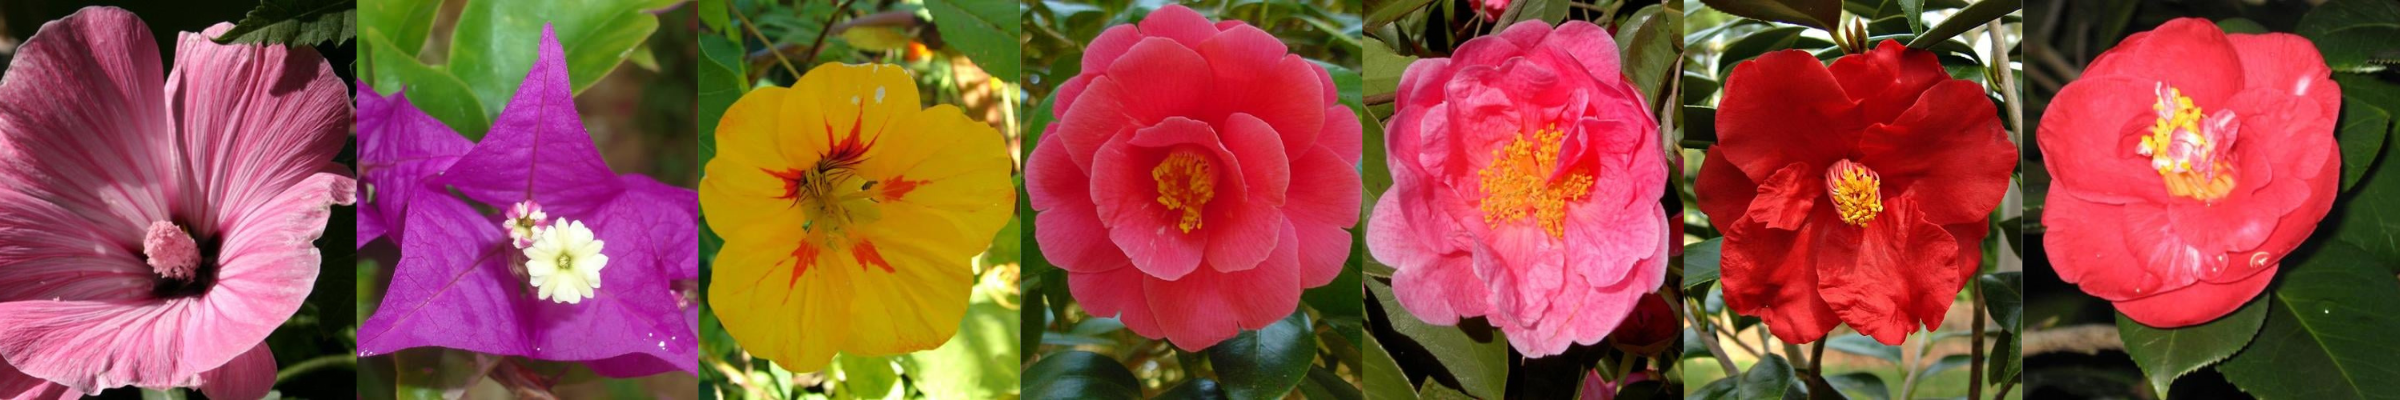
\includegraphics[width=0.9\linewidth]{images/flowers_dataset.png}
        \caption{\textit{Sample images from 102 Flower Dataset. Source \citep{Nilsback08}}}
        \label{fig:102Flower}
    \end{figure}

    Figure~\ref{fig:102Flower} shows sample images from the 102 Flower dataset, which comprises 102 flower classes present in the United Kingdom. There are between 40 and 258 images in each class. The flowers covered by the dataset are regularly occurring species in the UK. The dataset shows a great deal of variation in the sizes, pose, and lighting conditions of the flowers, which is an added complexity for the task of classification. Moreover, there are large intra-class differences for some categories, and there are many categories that are visually extremely similar to each other. All such attributes make the dataset extremely suitable for fine-grained visual categorization. The dataset was also used for analysis and visualization using isomap dimensionality reduction based on shape and color descriptors, which revealed the structure of the different flower categories. As for the sizes of the images, the raw images in the dataset are of varying sizes. For instance, one raw image from the dataset measures 500×667 pixels \citep{Nilsback08}.
    
\end{enumerate}

\subsection{Data Preprocessing Steps}

For all datasets, we will apply the following preprocessing steps:

\begin{itemize}
    \item Resizing and Normalization: Images will be resized to 256×256 for efficiency (and 512×512 for high-res experiments) and pixel values will be normalized to the range [-1,1] for input to StyleGAN2.
    \item Filtering: We will remove any extremely low-quality or mislabeled images.
    \begin{itemize}
        \item For FUNIT Animal Faces, use a face detector, MTCNN (Multi-Task Cascaded Convolutional Networks), to crop and horizontally align faces so the eyes are leveled.
    \end{itemize}

    \item Train-Test Splitting : We assess our approach on four standard few‐shot image domains, partitioning each into “seen” classes for model fitting and “unseen” classes for testing:
    
    \begin{itemize}
      \item \textbf{Animal Faces.} Out of the total categories, 120 are used as seen classes for training, while the remaining 30 serve as unseen classes for evaluation.
      \item \textbf{Flowers.} We assign 85 categories to the training (seen) split and reserve 15 categories for the test (unseen) split.
    \end{itemize}
    
    \item Augmentation: No data augmentation will be used beyond centering and flipping, since we focus on the evaluation of given domains. All datasets and preprocessing pipelines are documented for reproducibility.
\end{itemize}